%%%%%%%%%%%%%%%%%%%%%%%%%%%%%%%%%%%%%%%%%%%%%%%%%%%%%%%%%%%%%%%%
%%                                                            %%
%%   essentialsOfLatin, Italian translation 2017              %%
%%                                                            %%
%% From:  Henry C. Pearson, Essentials Of Latin For Beginners %%
%%        (1915, New York, American Book Company)             %%
%%                                                            %%
%%    https://archive.org/details/essentialslatin04peargoog   %%
%%                                                            %%
%% Translated by g.p.ciceri <gp.ciceri@gmail.com>             %%
%% ---------------------------------------------------------- %%
%% This translation is Licensed under                         %%
%% Creative Commons Attribution-ShareAlike 4.0 International  %%
%% https://creativecommons.org/licenses/by-sa/4.0/            %%
%%                                                            %%
%%%%%%%%%%%%%%%%%%%%%%%%%%%%%%%%%%%%%%%%%%%%%%%%%%%%%%%%%%%%%%%%

% āēīōū
% ăĕĭŏŭ




\documentclass[nols]{tufte-handout}

%\geometry{showframe} % display margins for debugging page layout

\usepackage{fontspec}
\usepackage{ifxetex}
\setmainfont[Path=./fonts/palatino-linotype/, ItalicFont=palai.ttf, BoldFont=palab.ttf]{pala.ttf}


% \defaultfontfeatures{Mapping=tex-text}
% \setromanfont[Path=./fonts/TeX-Gyre-Schola/,Mapping=tex-text]{TeX Gyre Schola}
% \setsansfont[Path=./fonts/TeX-Gyre-Heros/,Scale=MatchLowercase,Mapping=tex-text]{TeX Gyre Heros}
% \setmonofont[Path=./fonts/TeX-Gyre-Cursor/,Scale=MatchLowercase]{TeX Gyre Cursor}

\usepackage{lipsum}
\usepackage{url}
\usepackage{longtable}
\usepackage{stackengine}

\usepackage{graphicx} % allow embedded images
  \setkeys{Gin}{width=\linewidth,totalheight=\textheight,keepaspectratio}
  \graphicspath{{graphics/}} % set of paths to search for images
\usepackage{amsmath}  % extended mathematics
\usepackage{booktabs} % book-quality tables
\usepackage{units}    % non-stacked fractions and better unit spacing
\usepackage{multicol} % multiple column layout facilities
\usepackage{lipsum}   % filler text
\usepackage{fancyvrb} % extended verbatim environments
  \fvset{fontsize=\normalsize}% default font size for fancy-verbatim environments

% Standardize command font styles and environments
\newcommand{\doccmd}[1]{\texttt{\textbackslash#1}}% command name -- adds backslash automatically
\newcommand{\docopt}[1]{\ensuremath{\langle}\textrm{\textit{#1}}\ensuremath{\rangle}}% optional command argument
\newcommand{\docarg}[1]{\textrm{\textit{#1}}}% (required) command argument
\newcommand{\docenv}[1]{\textsf{#1}}% environment name
\newcommand{\docpkg}[1]{\texttt{#1}}% package name
\newcommand{\doccls}[1]{\texttt{#1}}% document class name
\newcommand{\docclsopt}[1]{\texttt{#1}}% document class option name
\newenvironment{docspec}{\begin{quote}\noindent}{\end{quote}}% command specification environment

% concetti morfosintattici
\usepackage{xspace} 
\newcommand{\noun}{\textsc{sostantivo}\xspace}
\newcommand{\nouns}{\textsc{sostantivi}\xspace}
\newcommand{\adject}{\textsc{aggettivo}\xspace}
\newcommand{\adjects}{\textsc{aggettivi}\xspace}
\newcommand{\gnumber}{\textsc{numero}\xspace}
\newcommand{\gnumbers}{\textsc{numeri}\xspace}
\newcommand{\gender}{\textsc{genere}\xspace}
\newcommand{\genders}{\textsc{generi}\xspace}
\newcommand{\gcase}{\textsc{caso}\xspace}
\newcommand{\gcases}{\textsc{casi}\xspace}
\newcommand{\tense}{\textsc{tempo}\xspace}
\newcommand{\mood}{\textsc{modo}\xspace}
\newcommand{\gverb}{\textsc{verbo}\xspace}
\newcommand{\gverbs}{\textsc{verbi}\xspace}
\newcommand{\adjective}{\textsc{aggettivo}\xspace}
\newcommand{\nom}{\textsc{nom}\xspace}
\newcommand{\gen}{\textsc{gen}\xspace}
\newcommand{\dat}{\textsc{dat}\xspace}
\newcommand{\acc}{\textsc{acc}\xspace}
\newcommand{\voc}{\textsc{voc}\xspace}
\newcommand{\abl}{\textsc{abl}\xspace}
\newcommand{\gexit}{\textsc{uscita}\xspace}
\newcommand{\gexits}{\textsc{uscite}\xspace}
\newcommand{\declinazione}{\textsc{declinazione}\xspace}
\newcommand{\masc}{\textsc{maschile}\xspace}
\newcommand{\femm}{\textsc{femminile}\xspace}
\newcommand{\neut}{\textsc{neutro}\xspace}

\newcommand{\indic}{\textsc{indicativo}\xspace}
\newcommand{\imper}{\textsc{imperativo}\xspace}
\newcommand{\gcong}{\textsc{congiuntivo}\xspace}
\newcommand{\ott}{\textsc{ottativo}\xspace}
\newcommand{\partic}{\textsc{participio}\xspace}
\newcommand{\infin}{\textsc{infinito}\xspace}

\newcommand{\pres}{\textsc{presente}\xspace}
\newcommand{\imperf}{\textsc{imperfetto}\xspace}
\newcommand{\aor}{\textsc{aoristo}\xspace}
\newcommand{\fut}{\textsc{futuro}\xspace}
\newcommand{\perf}{\textsc{perfetto}\xspace}
\newcommand{\pperf}{\textsc{piuccheperfetto}\xspace}

\newcommand{\sing}{\textsc{singolare}\xspace}
\newcommand{\plur}{\textsc{plurale}\xspace}
\newcommand{\dual}{\textsc{duale}\xspace}

\newcommand{\si}{\textsc{sing}\xspace}
\newcommand{\pl}{\textsc{plur}\xspace}
\newcommand{\du}{\textsc{dual}\xspace}

\newcommand{\att}{\textsc{attivo}\xspace}
\newcommand{\med}{\textsc{medio}\xspace}
\newcommand{\pass}{\textsc{passivo}\xspace}
\newcommand{\medpass}{\textsc{medio-passivo}\xspace}


% italianitudini
\renewcommand{\figurename}{Figura}
\renewcommand{\tablename}{Tabella}
\renewcommand{\contentsname}{Indice}

% fix per un qualche problema
\ifxetex
  \newcommand{\textls}[2][5]{%
    \begingroup\addfontfeatures{LetterSpace=#1}#2\endgroup
  }
  \renewcommand{\allcapsspacing}[1]{\textls[15]{#1}}
  \renewcommand{\smallcapsspacing}[1]{\textls[10]{#1}}
  \renewcommand{\allcaps}[1]{\textls[15]{\MakeTextUppercase{#1}}}
  \renewcommand{\smallcaps}[1]{\smallcapsspacing{\scshape\MakeTextLowercase{#1}}}
  \renewcommand{\textsc}[1]{\smallcapsspacing{\textsmallcaps{#1}}}
\fi

% too many float...
\extrafloats{100}

\title{Essentials Of Latin. Latino alle Medie. \newline Lezione XX - Presente Indicativo Passivo per la I e II coniugazione. Il Complemento d'Agente.}

\author[gpciceri]{a cura di Milagathòs: Milo's help to enjoy humanities.}

\date{20 Gennajo 2017} % without \date command, current date is supplied


\begin{document}

\hyphenation{co-niu-ga-zio-ne}

\maketitle% this prints the handout title, author, and date

\begin{marginfigure}[-2.5cm]
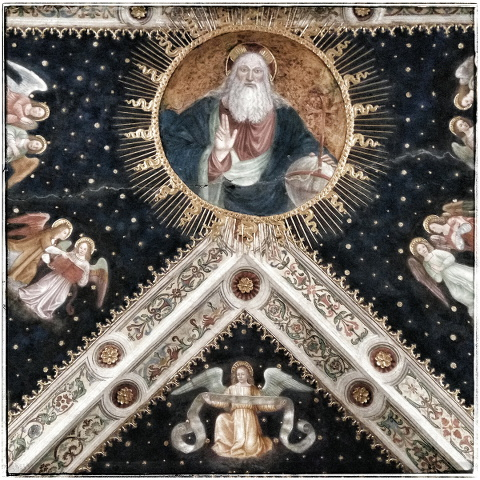
\includegraphics{smallthumb-lesson_XI.jpeg}
\setfloatalignment{b}
\end{marginfigure}


\begin{abstract}
\noindent
Queste lezioni riprendono il testo introduttivo al Latino di Pearson\cite{pearson1915}, del quale seguono la numerazione; la struttura di ogni lezione è piuttosto regolare: inizia con \textsc{cenni di morfologia e di sintassi latina}, seguita da un \textsc{piccolo vocabolario} per il lessico; ci sono infine vari \textsc{esercizi} di traduzione e di composizione latina.

\bigskip
\noindent
Lezione XX - Presente Indicativo Passivo per la I e II coniugazione. Il Complemento d'Agente.
\end{abstract}

%\printclassoptions

\newthought{138. Diatesi Attiva e Passiva.} Un verbo in diatesi attiva (in breve, all'attivo) vuol dire che il soggetto agisce, compie l'azione espressa dal verbo: \textit{l'agricoltore ara il campo, il fattore vive felicemente}; al passivo, invece, vuol dire che il soggetto subisce l'azione \textit{il campo è arato dall'agricoltore}. 

\newthought{139. Prima e Seconda Coniugazione, indicativo presente attivo e passivo.} 

\begin{fullwidth}
\begin{table}[!htbp]
  \centering
  \begin{tabular}{l l l l}
    %\toprule
	\multicolumn{4}{c}{\textsc{I Coniugazione - Diatesi Attiva, Indicativo Presente}} \\
	\multicolumn{3}{c}{\textsc{Singolare}} & \textsc{Terminazioni} \\

    \textsc{1.} & am\textbf{ō}, \textit{io amo}    & \hspace{20mm} & \textbf{-ō} \\
    \textsc{2.} & amā\textbf{s}, \textit{tu ami}   & \hspace{20mm} & \textbf{-s} \\
    \textsc{3.} & ama\textbf{t}, \textit{egli ama} & \hspace{20mm} & \textbf{-t} \\
	
	\multicolumn{3}{c}{\textsc{Plurale}} & \\
	
	\textsc{1.} & amā\textbf{mus}, \textit{noi amiamo} & \hspace{20mm} & \textbf{-mus} \\
    \textsc{2.} & amā\textbf{tis}, \textit{voi amate} & \hspace{20mm} & \textbf{-tis} \\
    \textsc{3.} & ama\textbf{nt}, \textit{essi amano}  & \hspace{20mm} & \textbf{-nt} \\
	
	\multicolumn{4}{c}{\textemdash} \\
	\multicolumn{4}{c}{\textsc{Diatesi Passiva, Indicativo Presente}} \\
	\multicolumn{3}{c}{\textsc{Singolare}} & \textsc{Terminazioni} \\

    \textsc{1.} & amo\textbf{r}, \textit{io sono amato}    & \hspace{20mm} & \textbf{-r} \\
    \textsc{2.} & amā\textbf{ris}, amā\textbf{re}, \textit{tu sei amato}    & \hspace{20mm} & \textbf{-ris, -re} \\
    \textsc{3.} & ama\textbf{tur}, \textit{egli è amato}   & \hspace{20mm} & \textbf{-tur} \\
	
	\multicolumn{3}{c}{\textsc{Plurale}} & \\
	
	\textsc{1.} & amā\textbf{mur}, \textit{noi siamo amati} & \hspace{20mm} & \textbf{-mur} \\
    \textsc{2.} & amā\textbf{minī}, \textit{voi siete amati} & \hspace{20mm} & \textbf{-minī} \\
    \textsc{3.} & ama\textbf{ntur}, \textit{essi sono amati}  & \hspace{20mm} & \textbf{-ntur} \\

    %\bottomrule
  \end{tabular}
  \caption{confronto tra le uscite personali della diatesi attiva e della diatesi passiva, Prima Coniugazione.}
  \label{tab:normaltab}
  %\zsavepos{pos:normaltab}
\end{table}
\end{fullwidth}

\begin{fullwidth}
\begin{table}[!htbp]
  \centering
  \begin{tabular}{l l l l}
    %\toprule
	\multicolumn{4}{c}{\textsc{II Coniugazione - Diatesi Attiva, Indicativo Presente}} \\
	\multicolumn{3}{c}{\textsc{Singolare}} & \textsc{Uscite} \\

    \textsc{1.} & mone\textbf{ō}, \textit{io ammonisco}    & \hspace{20mm} & \textbf{-ō} \\
    \textsc{2.} & monē\textbf{s}, \textit{tu ammonisci}   & \hspace{20mm} & \textbf{-s} \\
    \textsc{3.} & mone\textbf{t}, \textit{egli ammonisce} & \hspace{20mm} & \textbf{-t} \\
	
	\multicolumn{3}{c}{\textsc{Plurale}} & \\
	
	\textsc{1.} & monē\textbf{mus}, \textit{noi ammoniamo} & \hspace{20mm} & \textbf{-mus} \\
    \textsc{2.} & monē\textbf{tis}, \textit{voi ammonite} & \hspace{20mm} & \textbf{-tis} \\
    \textsc{3.} & mone\textbf{nt}, \textit{essi ammoniscono}  & \hspace{20mm} & \textbf{-nt} \\
	
	\multicolumn{4}{c}{\textemdash} \\
	\multicolumn{4}{c}{\textsc{Diatesi Passiva, Indicativo Presente}} \\
	\multicolumn{3}{c}{\textsc{Singolare}} & \textsc{Uscite} \\

    \textsc{1.} & moneo\textbf{r}, \textit{io sono ammonito}    & \hspace{20mm} & \textbf{-r} \\
    \textsc{2.} & monē\textbf{ris}, monē\textbf{re}, \textit{tu sei ammonito}    & \hspace{20mm} & \textbf{-ris, -re} \\
    \textsc{3.} & monē\textbf{tur}, \textit{egli è ammonito}   & \hspace{20mm} & \textbf{-tur} \\
	
	\multicolumn{3}{c}{\textsc{Plurale}} & \\
	
	\textsc{1.} & monē\textbf{mur}, \textit{noi siamo ammoniti} & \hspace{20mm} & \textbf{-mur} \\
    \textsc{2.} & monē\textbf{minī}, \textit{voi siete ammoniti} & \hspace{20mm} & \textbf{-minī} \\
    \textsc{3.} & mone\textbf{ntur}, \textit{essi sono ammoniti}  & \hspace{20mm} & \textbf{-ntur} \\
	
    %\bottomrule
  \end{tabular}
  \caption{confronto tra le uscite personali della diatesi attiva e della diatesi passiva, Seconda Coniugazione.}
  \label{tab:normaltab}
  %\zsavepos{pos:normaltab}
\end{table}
\end{fullwidth}

\newthought{Osservazioni}
\begin{itemize}
\item[\textsc{1.}] Confronta con cura le traduzioni in italiano delle forme attive e passive.  
\item[\textsc{2.}] Ripassa le uscite personali dell'attivo, e impare quelle del passivo.  
\item[\textsc{3.}] Osserva come queste uscite personali del passivo siano agganciate direttamente al tema verbale del presente \textbf{amā-} e \textbf{monē-}, tranne alla prima persona singolare.  
\end{itemize}


\newthought{140. Esercizio.} Coniuga il presente indicativo attivo e passivo, e traduci poi in italiano, i seguenti verbi.
\begin{multicols}{2}
    \noindent \hangindent=1em \textbf{laudō}, \textit{io lodo}.  \\
    \noindent \hangindent=1em \textbf{videō} \textit{io guardo}.  \\
    \noindent \hangindent=1em \textbf{vocō} \textit{io chiamo}.  \\
    \noindent \hangindent=1em \textbf{terreō} \textit{io spavento}.     \\
\end{multicols}

\newthought{141. Frasi Modello.} Esamina le seguenti frasi:
\begin{itemize}
\item[\textsc{1.}] \textbf{Coniurati Caesarem necant}, \textit{i congiurati uccidono Cesare}.  
\item[\textsc{2.}] \textbf{Caesar ā coniuratis necatur}, \textit{Cesare è ucciso dai congiurati}.  
\item[\textsc{3.}] \textbf{Caesar gladio necatur}, \textit{Cesare è ucciso da una spada}.    
\end{itemize}

\newpage

\newthought{Osservazioni.} Cambiamenti tra la forma attiva e quella passiva della frase:
\begin{itemize}
\item[\textsc{a.}] L'oggetto del verbo attivo diventa il soggetto del verbo al passivo;  
\item[\textsc{b.}] Il soggetto, cioè  \textit{chi agisce} o  \textit{chi fa}, del verbo attivo viene espresso, con il verbo al passivo, dall'ablativo con la preposizione \textbf{ā}.      
\end{itemize}

\newthought{(ripasso 93., 94.). Ablativo di mezzo o di Strumento, frasi modello} Esamina le seguenti frasi:
\begin{itemize}
\item[\textsc{1.}] \textbf{Hastis et sagittis pugnabant}, \textit{combattevano con lance e frecce}.  
\item[\textsc{2.}] \textbf{Equis frumentum portabimus}, \textit{porteremo il grano per mezzo di cavalli}.  
\end{itemize}
\newthought{Osservazione.} Confronta gli esempi 141.2 e 141.3: la preposizione \textbf{ā} è usata quando l'azione del verbo è compiuta da una persona, mentre non si usa quando l'azione è compiuta da una cosa - un agente non volontario insomma.

\newthought{142. Regola \textemdash Agente di un verbo passivo.} L'agente - se persona - di un'azione espressa da un verbo al passivo è espresso tramite il caso ablativo preceduto dala preposizione \textbf{ā} o \textbf{ab}.

\newthought{143. Vocabolario}

\begin{multicols}{2}
    \noindent \hangindent=1em \textbf{Caesar, -aris}, m., \textit{Cesare}.  \\
    \noindent \hangindent=1em \textbf{legio, -onis}, f., \textit{legione} (circa 5000 soldati).  \\
    \noindent \hangindent=1em \textbf{ā, ab},
	\marginnote{usa \textbf{ab} prima di una parola che inizi per vocale o per \textit{h}, 
	altrimenti usa \textbf{ā}.} prep. con \abl \textit{da, per mezzo di}.  \\
	\noindent \hangindent=1em \textbf{ob}, prep. con \acc \textit{per causa di, per}.     \\
    \noindent \hangindent=1em \textbf{celeritas, -atis} \textit{corpo}.  \\
    \noindent \hangindent=1em \textbf{incito, -as, -avi, -atum, -are} \textit{incitare, incoraggiare, suscitare}.  \\
    \noindent \hangindent=1em \textbf{ē, ex}, prep. con \abl \textit{da, per mezzo di}.  \\
    \noindent \hangindent=1em \textbf{propter}, prep. con \acc \textit{per causa di, per}.     \\
	
\end{multicols}

\newthought{Ripassare i verbi di (100.), (108.)}

\newthought{(verbi 100.)}

\begin{multicols}{2}
    \noindent \hangindent=1em \textbf{laudo, -as, -avi, -atum, -are} \textit{lodare, apprezzare}.  \\
    \noindent \hangindent=1em \textbf{voco, -as, -avi, -atum, -are} \textit{chiamare}.  \\
    \noindent \hangindent=1em \textbf{paro, -as, -avi, -atum, -are} \textit{preparare}.  \\
    \noindent \hangindent=1em \textbf{oppugno, -as, -avi, -atum, -are} \textit{assalire, espugnare}.  \\
    \noindent \hangindent=1em \textbf{servo, -as, -avi, -atum, -are} \textit{salvare, conservare}.  \\
	\noindent \hangindent=1em \textbf{culpo, -as, -avi, -atum, -are} \textit{criticare, accusare, incolpare}.  \\
    \noindent \hangindent=1em \textbf{convoco, -as, -avi, -atum, -are} \textit{convocare, riunire}.  \\
    \noindent \hangindent=1em \textbf{do, -as, dedi, -atum, -are} \textit{dare}.  \\
    \noindent \hangindent=1em \textbf{porto, -as, -avi, -atum, -are} \textit{portare, trasportare, sopportare}.  \\
    \noindent \hangindent=1em \textbf{supero, -as, -avi, -atum, -are} \textit{superare, vincere}.  \\
    
\end{multicols}

\newthought{(verbi 108.)}

\begin{multicols}{2}
    \noindent \hangindent=1em \textbf{moneo, -es, monui, monitum, monere} \textit{ammonire, mettere in guardia}.  \\
    \noindent \hangindent=1em \textbf{habeo, -es, habui, habitum, habere} \textit{avere, tenere}.  \\
    \noindent \hangindent=1em \textbf{video, -es, vidi, visum, videre} \textit{guardare}.  \\
    \noindent \hangindent=1em \textbf{terreo, -es, terrui, territum, terrere} \textit{atterrire, spaventare}.  \\
    \noindent \hangindent=1em \textbf{moveo, -es, movi, motum, movere} \textit{muovere}; \textbf{castra movere}, \textit{smontare l'accampamento}.  \\
    \noindent \hangindent=1em \textbf{dimico, -as, -avi, -atum, -are} \textit{combattere, contendere}.  \\
\end{multicols}


\newthought{144. Esercizi di Ripasso}
\\
\textsc{I.} \quad
\textsc{1.}~Romani hieme et aestate cum hostibus pugnabant. \quad
\textsc{2.}~Telis Romani hostes in fugam dederunt. \quad
\textsc{3.}~Quattuor annis multas navis in mari viderant. \quad
\textsc{4.}~Copias in castra multa nocte consul convocavit. \quad
\textsc{5.}~Pons in flumine erat. \quad
\textsc{6.}~Caede liberorum miserorum miseri sumus.
\\
\textsc{II.} \quad
\textsc{1.}~In estate le giorante sono lunghe. \quad
\textsc{2.}~La cavalleria di Cesare prese possesso della collina all'alba. \quad
\textsc{3.}~Ci sono molte navi sul mare. \quad
\textsc{4.}~I romani non soffrirono la mancanza di condottieri.

\newthought{145. Esercizi}
\\
\textsc{I.} \quad
\textsc{1.}~Laudat, laudatur; videtis, videmini. \quad
\textsc{2.}~Incitant, incitantur; vocamus, vocamur. \quad
\textsc{3.}~Caesar milites convocat. \quad
\textsc{4.}~Milites a Caesare convocantur. \quad
\textsc{5.}~Dux legionem ob virtutem laudat. \quad
\textsc{6.}~Legio a duce propter virtutem laudatur. \quad
\textsc{7.}~Hostes celeritate equitum terrentur. \quad
\textsc{8.}~Magna cibi copia a militibus in castra portatur. \quad
\textsc{9.}~Virtute militum incolae oppidi incitantur. \quad
\textsc{10.}~Ex agris frumentum a militibus in hiberna portatur. \quad
\textsc{11.}~Multa nocte a pedite gladio vulteratur. \quad
\\
\textsc{II.} \quad
\textsc{1.}~Siamo convocati; egli chiama; egli è chiamato. \quad
\textsc{2.}~Voi incolpate; siete incolpati. \quad
\textsc{3.}~La rapidità dei Romani spaventa i Galli. \quad
\textsc{4.}~I Galli sono spaventati dalla rapidità dei Romani. \quad
\textsc{5.}~Cesare incoraggia i soldati. \quad
\textsc{6.}~I soldati sono incoraggiati da Cesare. \quad
\textsc{7.}~Sono convocati dai monti in città \textit{(a venire in città)} attraverso i campi.

\begin{figure*}[!b]
  %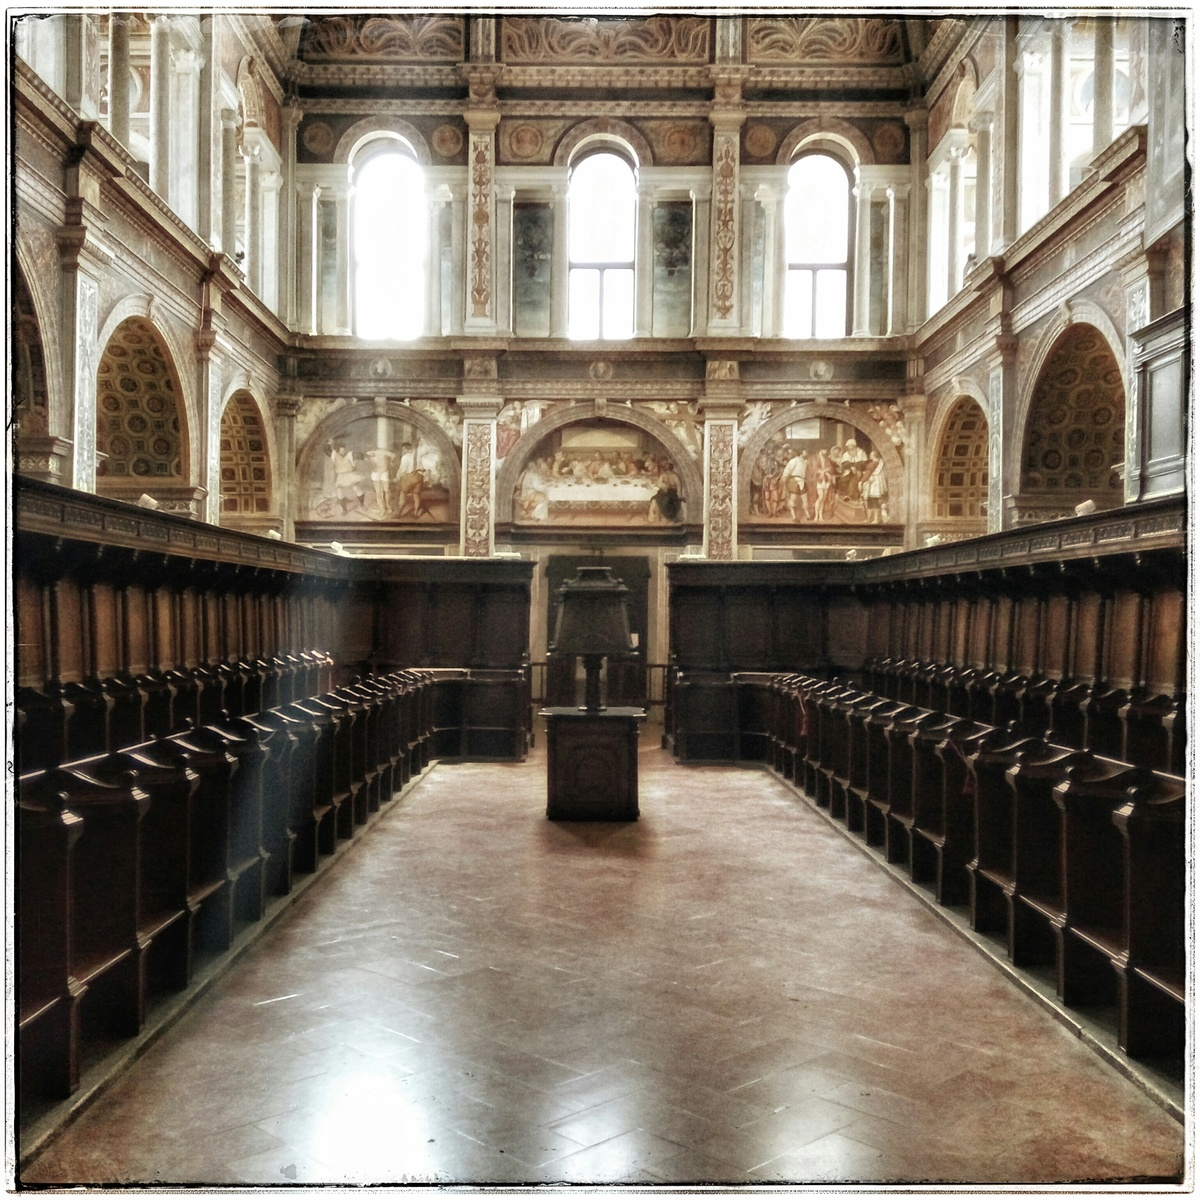
\includegraphics{thumb-lesson_XX.jpeg}
  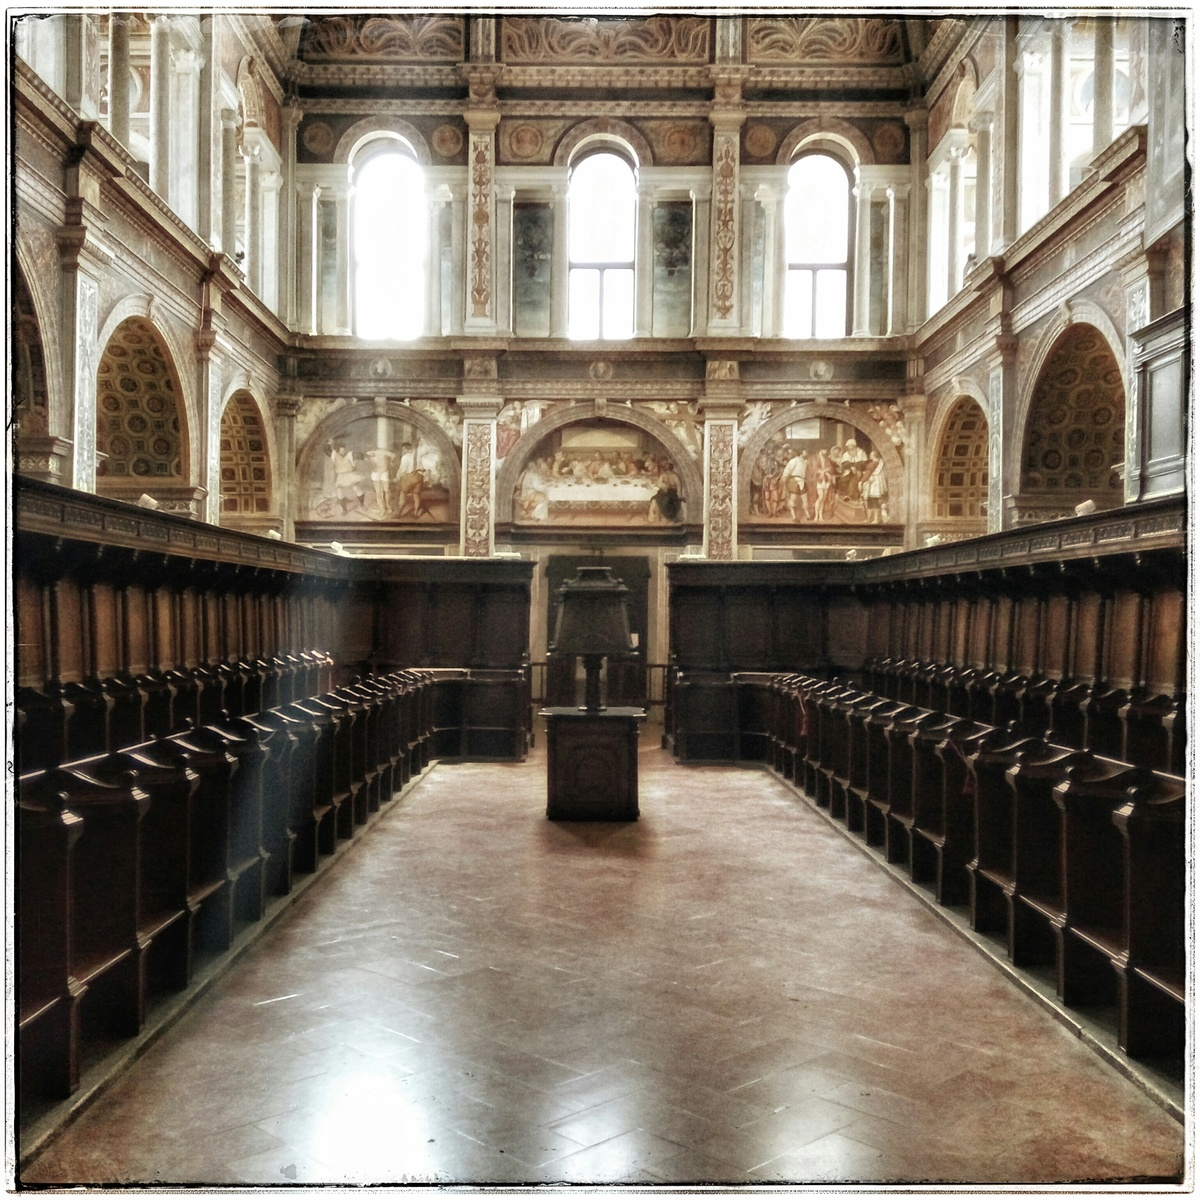
\includegraphics[width=0.8\linewidth]{thumb-lesson_XX.jpeg}
  %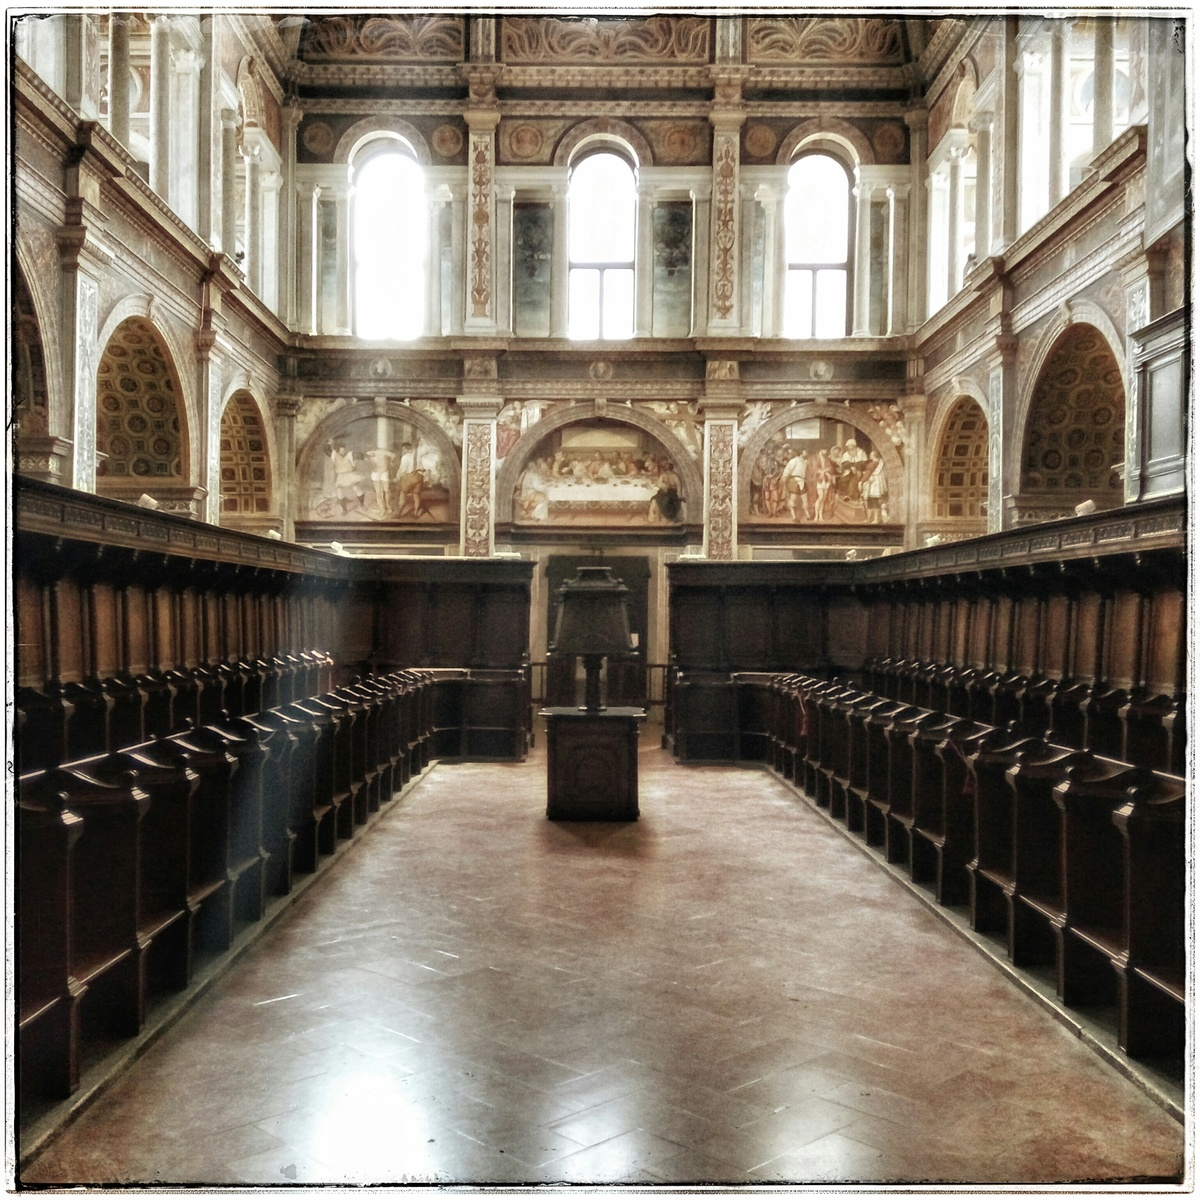
\includegraphics{thumb-lesson_XX.jpeg}
  \caption{Milano: San Maurizio al Monastero Maggiore}
  \label{fig:textfig}
  %\zsavepos{pos:textfig}
  %\setfloatalignment{b}
\end{figure*}

 

\nobibliography{latinBiblio}
\bibliographystyle{alpha}


\end{document}
